\documentclass[10pt,a4paper]{article}

\usepackage[a4paper,margin=2cm]{geometry}
\usepackage{graphicx}
\usepackage{float}
\usepackage{booktabs}
\usepackage{amsmath}
\usepackage{microtype}
\usepackage{cite}
\usepackage[section]{placeins}
\usepackage[hidelinks]{hyperref}

\setlength{\parindent}{0pt}
\setlength{\parskip}{0.45em}
\setlength{\textfloatsep}{10pt plus 2pt minus 2pt}
\setlength{\floatsep}{8pt plus 2pt minus 2pt}
\setlength{\intextsep}{8pt plus 2pt minus 2pt}
\setlength{\abovecaptionskip}{5pt}
\setlength{\belowcaptionskip}{3pt}
\setlength{\abovedisplayskip}{0.45em plus 0.15em minus 0.15em}
\setlength{\belowdisplayskip}{0.45em plus 0.15em minus 0.15em}
\setlength{\abovedisplayshortskip}{0.3em plus 0.1em minus 0.1em}
\setlength{\belowdisplayshortskip}{0.3em plus 0.1em minus 0.1em}
\setlength{\emergencystretch}{2em}

\makeatletter
\renewcommand\section{\@startsection{section}{1}{\z@}%
  {1em plus .25em minus .15em}{0.45em plus .1em}%
  {\normalfont\Large\bfseries}}
\renewcommand\subsection{\@startsection{subsection}{2}{\z@}%
  {0.75em plus .2em minus .1em}{0.25em plus .1em}%
  {\normalfont\large\bfseries}}
\renewcommand\subsubsection{\@startsection{subsubsection}{3}{\z@}%
  {0.55em plus .15em minus .1em}{0.2em plus .05em}%
  {\normalfont\normalsize\bfseries}}
\def\@listi{\leftmargin\leftmargini
  \topsep 0.2em plus 0.05em minus 0.05em
  \parsep 0.08em plus 0.03em minus 0.03em
  \itemsep 0.08em plus 0.03em minus 0.03em}
\let\@listI\@listi
\@listi
\def\@listii{\leftmargin\leftmarginii
  \topsep 0.15em plus 0.05em minus 0.05em
  \parsep 0.05em plus 0.02em minus 0.02em
  \itemsep 0.05em plus 0.02em minus 0.02em}
\makeatother

\title{Impact of JPEG Recompression and WebP Transcoding on Image Classification Performance}
\author{Author: Rimsha Afzal\\Course: Signal, Image and Video\\University of Trento}
\date{}

\begin{document}

\maketitle

\begin{abstract}
Lossy image compression is widely used to reduce storage and transmission costs, but its effects in machine-perception pipelines must be evaluated beyond visual distortion alone. This project studies JPEG recompression and JPEG-to-WebP transcoding on the Imagenette and ImageWoof validation sets using a frozen ImageNet-pretrained ResNet-50 classifier. For each dataset, codec, and quality condition, the experiment measures compression ratio, PSNR, SSIM, and top-1 accuracy. Using a primary acceptable accuracy loss of 1 percentage point, JPEG q70 is identified as the strongest tested JPEG condition passing the primary tolerance on both datasets, while WebP q80 is the strongest tested WebP condition passing the same rule. WebP q77 is an informative near-boundary condition, reducing size by approximately 20--21\% while retaining mean SSIM close to 0.96, but slightly exceeding the primary accuracy-loss tolerance. Within this experiment, WebP provides the strongest observed rate--accuracy trade-off among the tested passing settings, without implying an exact continuous optimum or universal codec superiority.
\end{abstract}

\section{Introduction}

Lossy image compression reduces storage and transmission requirements by discarding image information that is considered less important for reconstruction. This makes it useful in image archives, web applications, edge systems, and machine-perception pipelines where large numbers of images must be stored, transmitted, or processed efficiently.

However, perceptual image quality and classifier performance are not necessarily equivalent. Metrics such as PSNR and SSIM measure distortion relative to a reference image, but they do not directly show whether a classifier preserves the same correct decisions. Compression should therefore be evaluated jointly in terms of storage reduction, image distortion, and downstream classification performance. Previous work has shown that JPEG compression can reduce storage without necessarily degrading pretrained image-classification performance, while learned compression has also been designed explicitly for machine-perception tasks \cite{yang2021compression,codevilla2021learned}. Luo et al. formalized the joint rate--distortion--accuracy trade-off; in contrast, this study evaluates fixed JPEG and WebP settings using decoded images and a frozen classifier \cite{luo2021rda}.

At a signal-processing level, JPEG uses block-based transform coding: image blocks are transformed into frequency coefficients, quantization removes or coarsens information more strongly at lower quality settings, and entropy coding represents the resulting coefficients efficiently. Lossy WebP also combines block-based prediction, transform coding, quantization, and entropy coding, but with a different coding architecture. Because the quality numbers are encoder-specific, JPEG and WebP are compared here through achieved compression ratio, size reduction, decoded-image distortion, and classification performance rather than equal numerical quality settings.

\subsection{Research Objective}

The main objective of this project is to investigate how increasing JPEG recompression and JPEG-to-WebP transcoding affect storage size, decoded image quality, and frozen ResNet-50 top-1 classification performance on Imagenette and ImageWoof.

A second objective is to identify a practical compression threshold as the strongest tested compression condition that keeps classification degradation within a predefined acceptable accuracy-loss tolerance. This threshold is not universal. It depends on the dataset, codec, classifier, preprocessing pipeline, and selected acceptable-loss tolerance.

\subsection{Research Questions}

The project is guided by the following research questions:

\begin{description}
    \item[(i)] How does increasing lossy compression affect storage reduction, decoded-image distortion, and frozen ResNet-50 top-1 classification accuracy?
    \item[(ii)] At approximately comparable storage reductions, how do JPEG recompression and JPEG-to-WebP transcoding differ in their preservation of image quality and classification performance?
    \item[(iii)] For each dataset and codec, what is the strongest tested compression condition that reduces file size while keeping classification loss within the predefined acceptable tolerance?
\end{description}

The exploratory and targeted-refinement stages jointly address all three research questions.

\section{Methodology}

\subsection{Datasets and Target Classes}

The experiment uses the validation splits of Imagenette and ImageWoof, two
ten-class subsets derived from ImageNet \cite{fastai_imagenette,deng2009imagenet}. Imagenette contributes 3,925 evaluated
images, while ImageWoof contributes 3,929 evaluated images. The training splits
are not used.

Imagenette contains heterogeneous object categories:

\[
\mathcal{C}_{\text{Imagenette}} =
\left[
\begin{array}{lllll}
\text{tench}, &
\text{English springer}, &
\text{cassette player}, &
\text{chain saw}, &
\text{church}, \\
\text{French horn}, &
\text{garbage truck}, &
\text{gas pump}, &
\text{golf ball}, &
\text{parachute}
\end{array}
\right].
\]

ImageWoof contains ten visually related dog categories and therefore represents
a more fine-grained classification task:

\[
\mathcal{C}_{\text{ImageWoof}} =
\left[
\begin{array}{llll}
\text{Australian terrier}, &
\text{Border terrier}, &
\text{Samoyed}, &
\text{Beagle}, \\
\text{Shih-Tzu}, &
\text{English foxhound}, &
\text{Rhodesian ridgeback}, &
\text{Dingo}, \\
\text{Golden retriever}, &
\text{Old English sheepdog}
\end{array}
\right].
\]

Although each dataset contains only ten target categories, classification is
performed in the original 1,000-class ImageNet output space of the pretrained
ResNet-50. The model output is not restricted to the ten subset classes. Each
dataset label is mapped to its corresponding ImageNet class index, and a
prediction is counted as correct only when the top-1 prediction among all
1,000 output classes matches the mapped target.
\subsection{Experimental Framing}

The distributed source images are already JPEG encoded. The baseline condition is therefore the original distributed JPEG image, not a raw or lossless source image. JPEG conditions represent additional JPEG recompression after decoding the distributed image, while WebP conditions represent JPEG-to-WebP transcoding. Consequently, the experiment is not a comparison starting from raw or lossless image sources. PSNR and SSIM use the decoded distributed JPEG pixels as the reference.

\subsection{Baseline Classifier}

Classification is performed with an ImageNet-pretrained ResNet-50 \cite{he2016resnet} using the \texttt{IMAGENET1K\_V2} weights. The model parameters are frozen, the model is placed in evaluation mode, and no training or fine-tuning is performed. Images are processed with the official torchvision preprocessing associated with the selected ResNet-50 weights. Predictions are made in the original 1,000-class ImageNet output space \cite{torchvision_resnet50}.

\subsection{Compression and Classification Pipeline}

For each validation image, the implemented pipeline proceeds as follows:

\begin{enumerate}
    \item Load the distributed JPEG image.
    \item Decode it to RGB.
    \item Encode it in memory using JPEG or WebP.
    \item Apply the codec-quality conditions defined in the exploratory and targeted refinement stages.
    \item Record the encoded byte size.
    \item Decode the compressed result.
    \item Compute PSNR and SSIM against the decoded source image.
    \item Apply the same ResNet-50 preprocessing.
    \item Classify the compressed image.
    \item Save one result per image, codec, and quality.
\end{enumerate}

The compressed images are encoded and decoded in memory for measurement and inference; the implementation stores the resulting per-image measurements and predictions rather than storing a compressed image dataset.

\subsubsection{Implementation and Encoder Configuration}

The experiments were run with Python 3.12.13, PyTorch 2.12.1+cpu, torchvision 0.27.1+cpu, Pillow 12.2.0, and scikit-image 0.26.0. Each source image is opened with Pillow, converted to RGB, encoded in memory, decoded again, and converted to RGB before metric computation and classification. Encoder defaults and metadata choices are documented because they can affect encoded byte size.

\begin{sloppypar}
\begin{itemize}
    \item JPEG and WebP encoding use Pillow \texttt{Image.save}; the only explicitly configured encoder argument is \texttt{quality}.
    \item JPEG chroma subsampling, \texttt{optimize}, and \texttt{progressive} use Pillow defaults. WebP lossless mode, method, and other encoder options also use Pillow defaults.
    \item EXIF data, ICC profiles, thumbnails, and other metadata are not passed to the in-memory save calls and are not intentionally retained.
    \item PSNR uses scikit-image \texttt{peak\_signal\_noise\_\allowbreak ratio}; SSIM uses \texttt{structural\_\allowbreak similarity} with \texttt{channel\_axis=-1}. Both use \texttt{data\_range=255} on RGB arrays, and reported values are arithmetic means over images.
\end{itemize}
\end{sloppypar}

\subsection{Metrics}

\subsubsection{Compression Ratio}

The aggregate compression ratio is defined as
\[
\text{compression ratio} =
\frac{\text{total original size}}{\text{total compressed size}}.
\]
A ratio above 1 means that the compressed output is smaller than the source files, a ratio equal to 1 means no size change, and a ratio below 1 means that the compressed output is larger.

\subsubsection{Size Reduction}

Size reduction is defined as
\[
\text{size reduction} =
\left(1 - \frac{\text{total compressed size}}{\text{total original size}}\right)
\times 100.
\]
Negative values mean that the recompressed or transcoded output is larger than the distributed source files.

\subsubsection{PSNR and SSIM}

PSNR is derived from the mean squared reconstruction error:
\[
\mathrm{PSNR} = 10 \log_{10}\left(\frac{MAX_I^2}{\mathrm{MSE}}\right).
\]
In this implementation, \(MAX_I = 255\), matching the RGB pixel range used by the scikit-image metric calls. PSNR summarizes pixel-level reconstruction error, while SSIM compares local structural characteristics such as luminance, contrast, and structure \cite{wang2004ssim}. Higher values indicate greater similarity to the decoded distributed JPEG source reference. Neither metric directly measures classification performance.

\subsubsection{Classification Accuracy}

Baseline top-1 accuracy is measured on the original distributed validation images. Compressed top-1 accuracy is measured after JPEG recompression or WebP transcoding. Accuracy change is reported in percentage points:
\[
\text{accuracy change} =
\text{compressed accuracy} - \text{baseline accuracy}.
\]
Negative values indicate classification degradation relative to the baseline.

\subsection{Exploratory Experimental Stage}

The quality values 95, 80, 60, 40, 20, and 10 form a broad exploratory grid. The purpose of this grid is to observe the general rate--distortion--accuracy relationship, identify conditions that do not produce useful storage reduction, and locate the transition between mild and more pronounced classification degradation. This sparse grid supports targeted refinement but is not intended to identify an exact continuous threshold by itself.

\subsection{Targeted Refinement Stage}

The exploratory results indicated different transition regions for JPEG and WebP. Therefore, one additional codec-specific quality was evaluated for each codec: JPEG q70 and WebP q77. Both conditions were tested on Imagenette and ImageWoof using the same compression, distortion-measurement, preprocessing, and classification pipeline as the exploratory conditions. Different quality values were selected because JPEG and WebP quality scales are not directly equivalent. The purpose of this stage was to refine the observed transition around the predefined accuracy-loss tolerance without attempting to estimate an exact continuous optimum.

\subsection{Threshold-Identification Method}

The primary acceptable loss in top-1 accuracy is set to 1 percentage point relative to the original baseline. The 1 percentage-point value is an engineering tolerance selected for this experiment rather than a statistical-significance threshold or a universal machine-perception standard. Results are also examined using 0.5 and 2 percentage points as stricter and more permissive sensitivity cases that show how the selected operating point changes with the accepted loss.

For each dataset and codec, a tested condition qualifies only if it produces a compression ratio above 1 and keeps accuracy loss within the selected tolerance. The practical threshold is defined as the qualifying condition with the largest observed compression ratio. Because only discrete codec-quality settings are evaluated, this represents a practical point-estimate threshold rather than an exact continuous optimum. Compression ratio and size reduction describe the selected operating point, while PSNR and SSIM characterize the corresponding decoded-image distortion.

\section{Results}

\subsection{Baseline Overview}

The baseline evaluation includes 3,925 Imagenette validation images, with a top-1 accuracy of 87.18\% and a total source size of 97.81 MiB. ImageWoof includes 3,929 validation images, with a baseline accuracy of 88.27\% and a total source size of 96.71 MiB.

\subsection{Imagenette Results}

For Imagenette, JPEG q95 and q80 and WebP q95 produce outputs larger than the distributed source files, despite retaining accuracy close to the baseline. The first tested JPEG condition providing useful storage reduction is q60, which reduces total size by 11.2\% and changes accuracy by $-1.30$ percentage points. WebP q80 provides a similar size reduction of 12.9\% with a smaller observed accuracy change of $-0.84$ percentage points. At stronger compression levels, both codecs show progressively lower PSNR, SSIM, and classification accuracy.

\subsection{ImageWoof Results}

For ImageWoof, JPEG q95 and q80 and WebP q95 also increase the total file size. At approximately similar mild compression levels, JPEG q60 reduces storage by 10.6\% with an observed accuracy change of $-1.58$ percentage points, while WebP q80 reduces storage by 11.9\% with a smaller observed change of $-0.74$ percentage points. Accuracy degradation becomes more pronounced under aggressive compression: JPEG q10 changes accuracy by $-16.42$ percentage points, compared with $-10.66$ percentage points for WebP q10.

\begin{table}[!htbp]
    \centering
    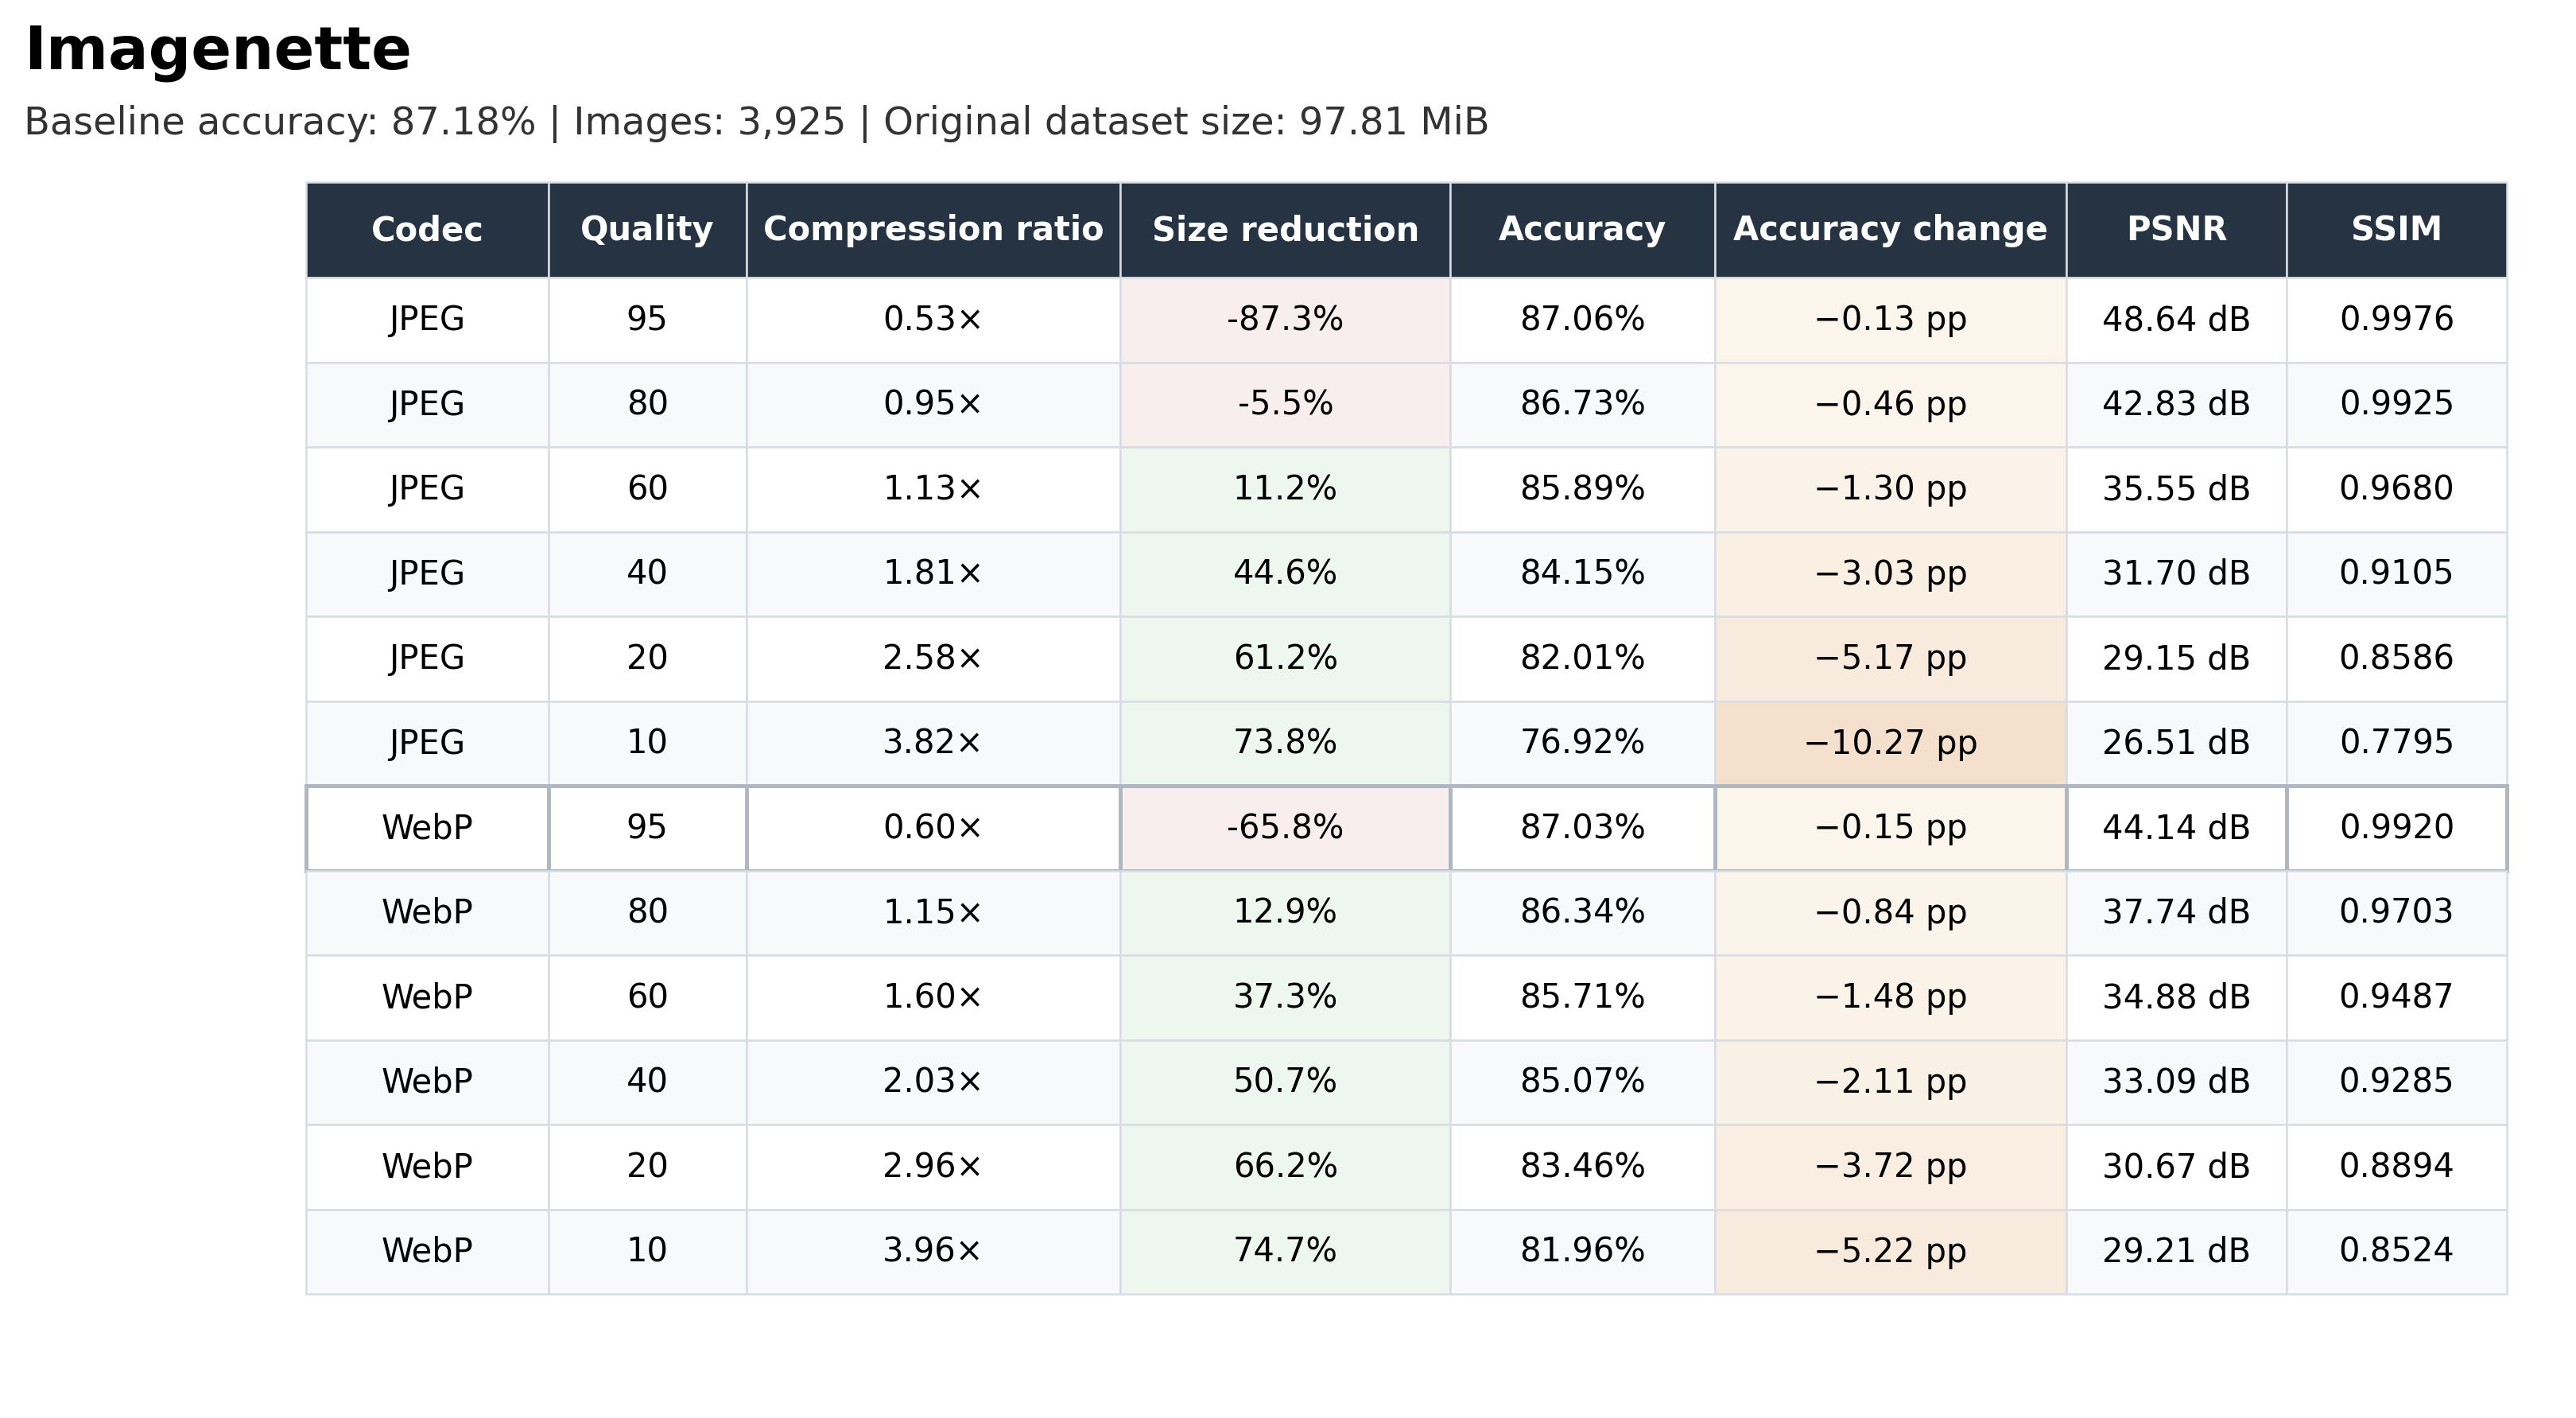
\includegraphics[width=0.90\textwidth]{../results/analysis/tables/imagenette_results_table.png}
    \caption{Imagenette aggregate rate--distortion--accuracy results for JPEG recompression and WebP transcoding.}
    \label{tab:imagenette-results}
\end{table}

\begin{table}[!htbp]
    \centering
    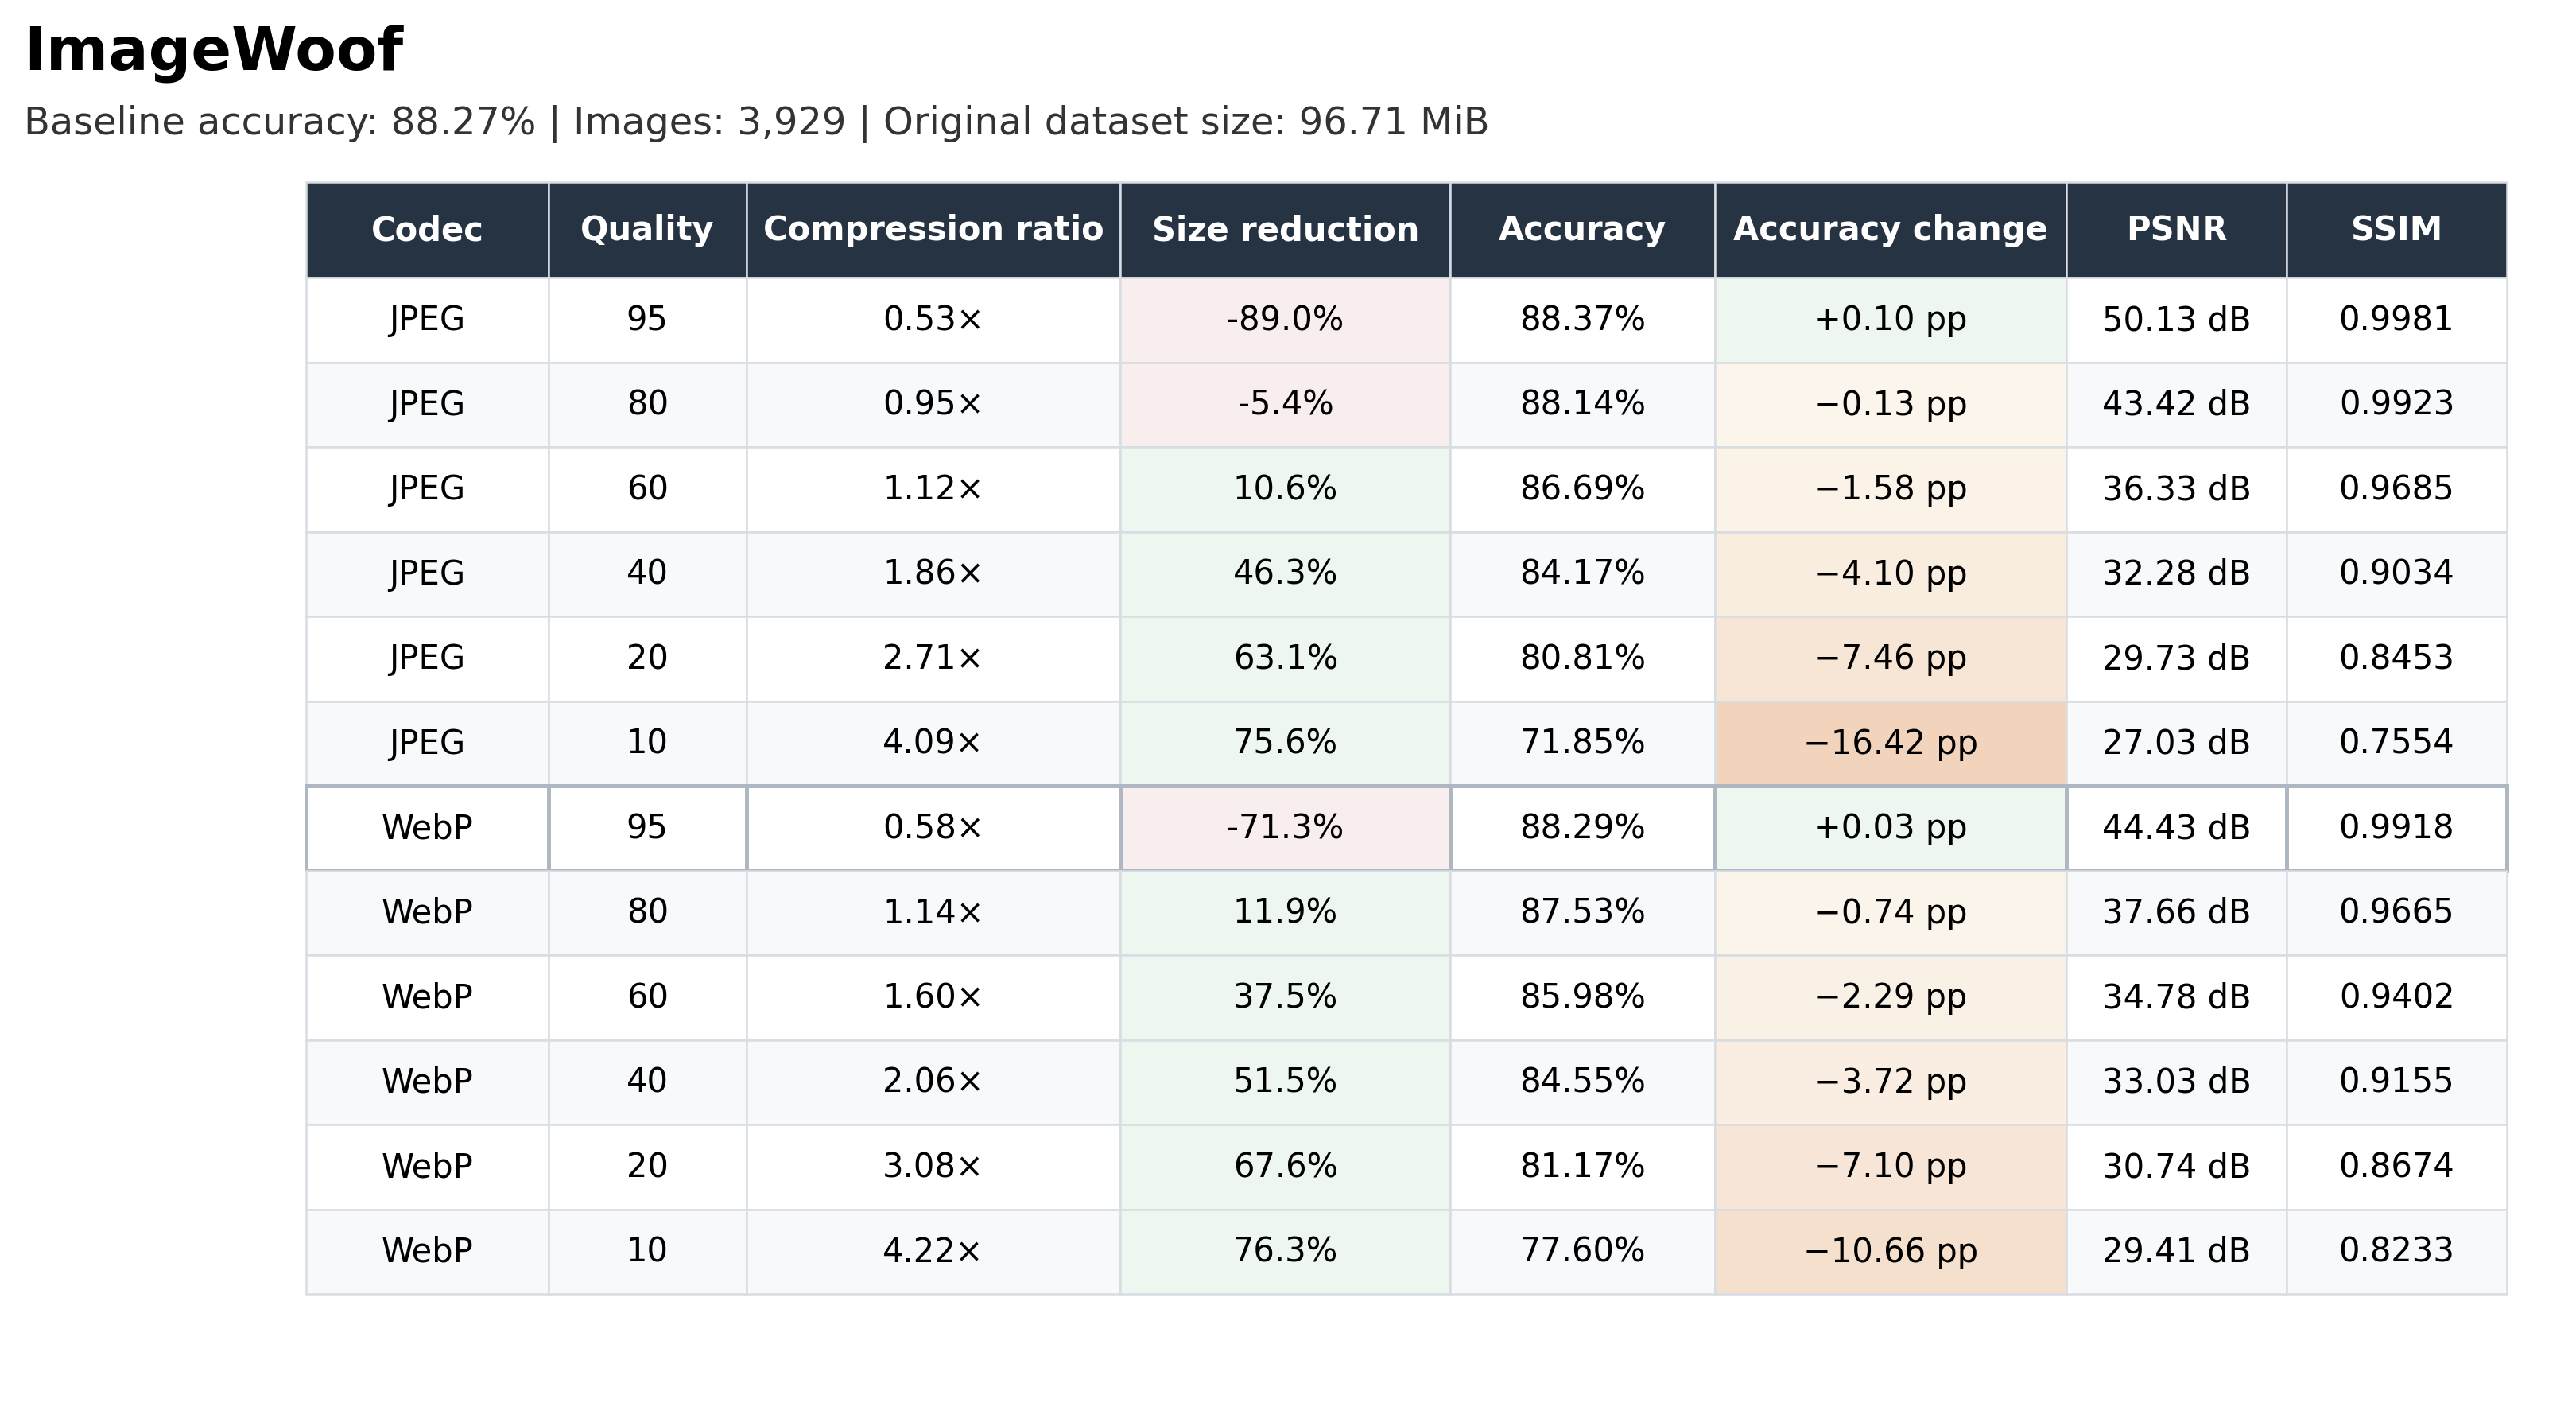
\includegraphics[width=0.90\textwidth]{../results/analysis/tables/imagewoof_results_table.png}
    \caption{ImageWoof aggregate rate--distortion--accuracy results for JPEG recompression and WebP transcoding.}
    \label{tab:imagewoof-results}
\end{table}

\FloatBarrier

\subsection{Rate--Accuracy Trade-off}

\begin{figure}[!htbp]
    \centering
    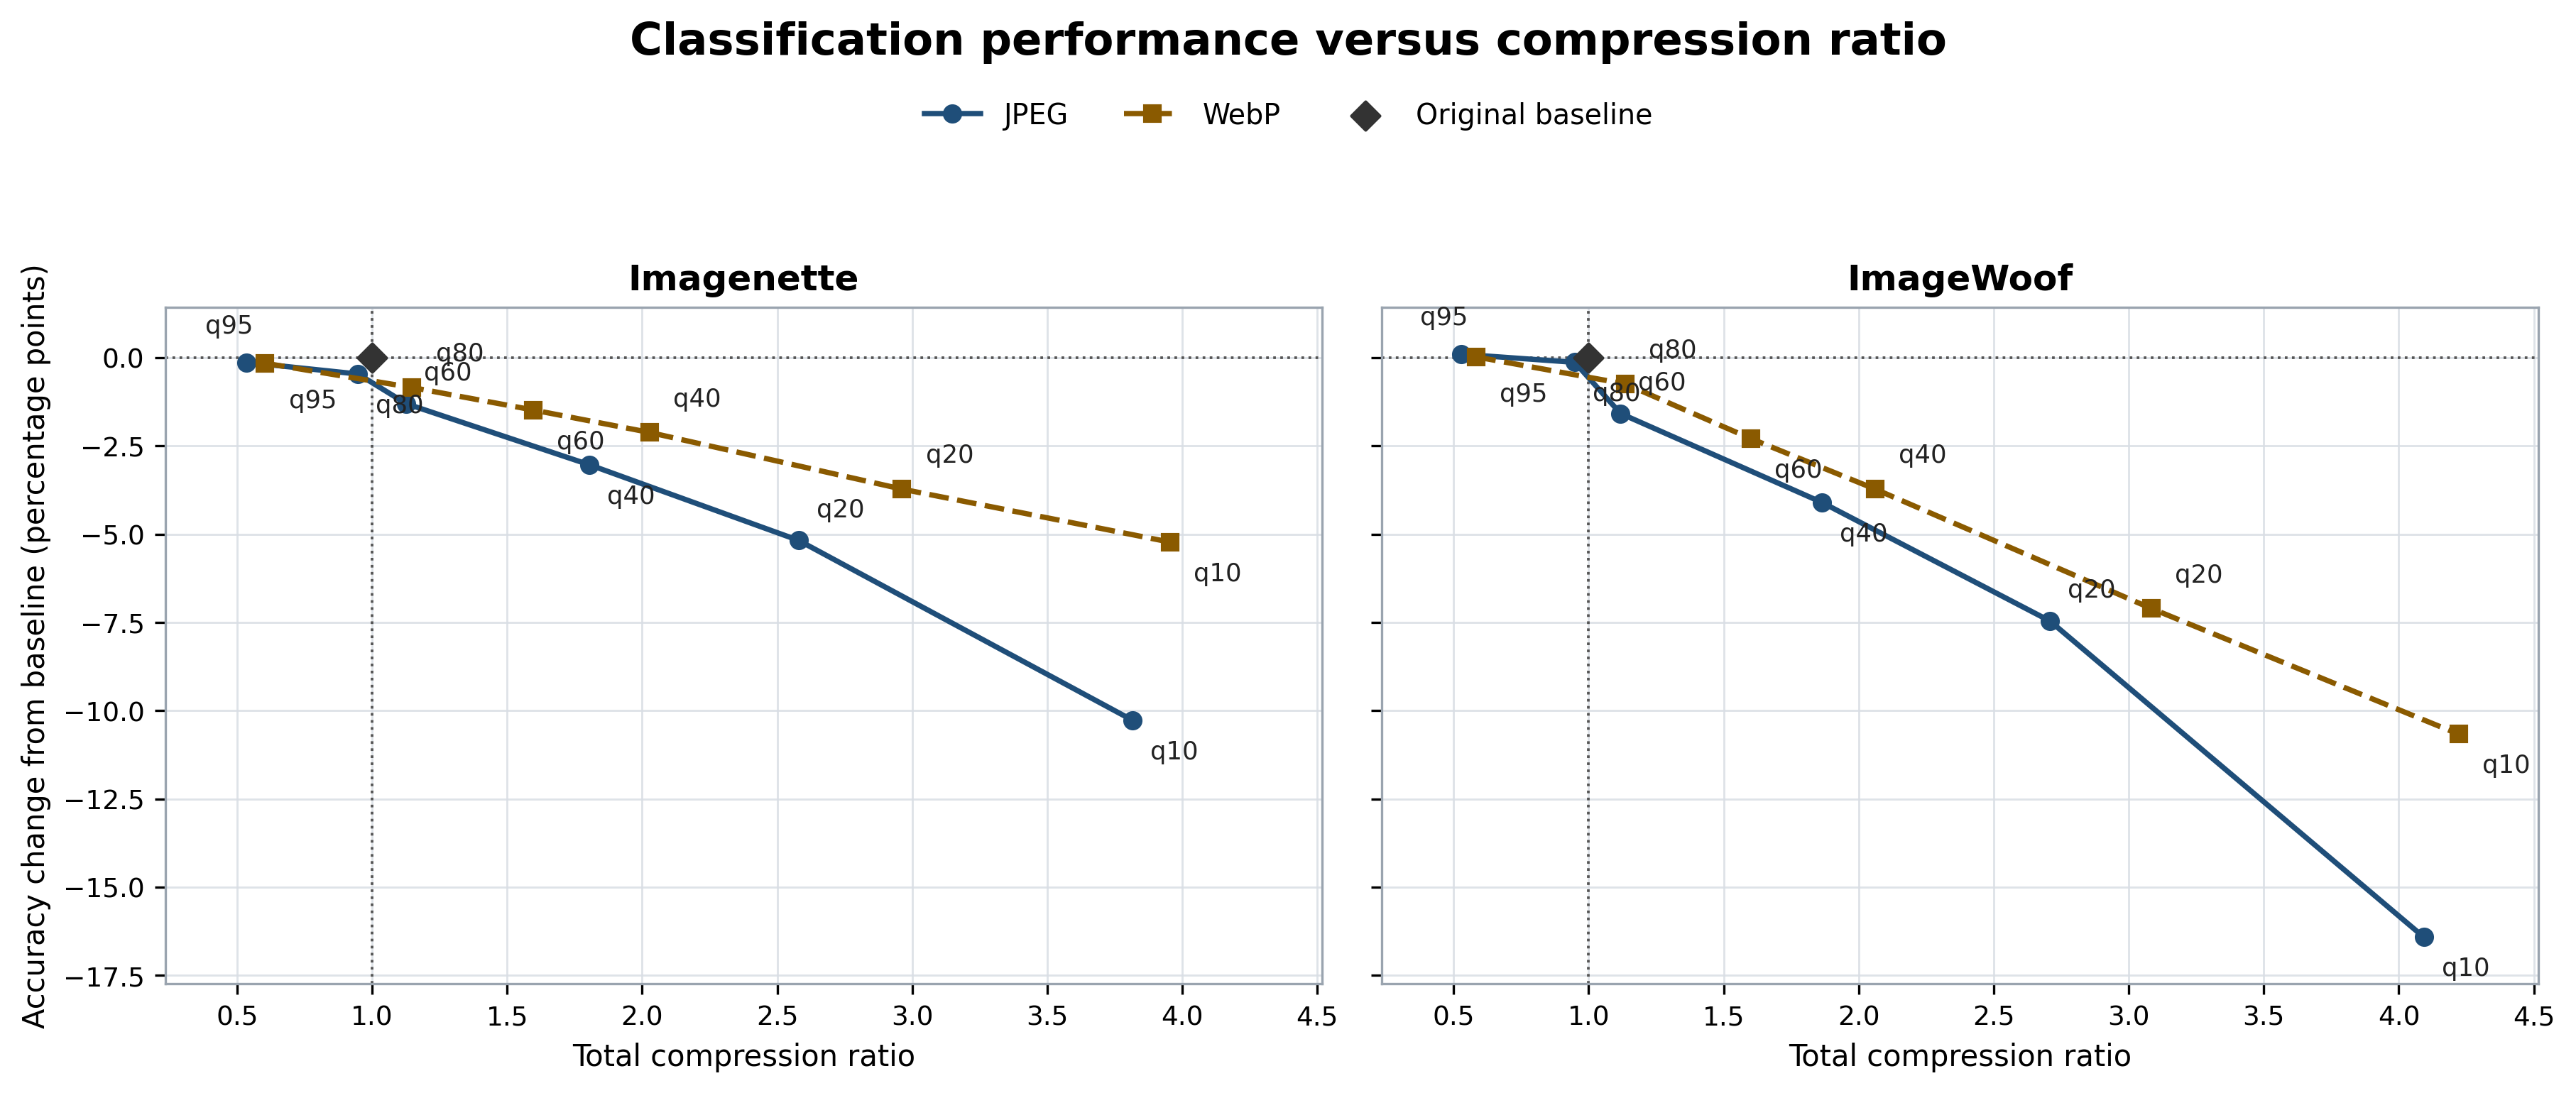
\includegraphics[width=0.92\textwidth]{../results/analysis/plots/rate_accuracy_tradeoff.png}
    \caption{Top-1 accuracy change relative to the original distributed JPEG baseline as a function of total compression ratio. Ratios below one indicate that recompression or transcoding increased the total file size.}
    \label{fig:rate_accuracy}
\end{figure}

Figure~\ref{fig:rate_accuracy} shows that conditions with compression ratios below 1 produce outputs larger than the source files. These conditions preserve accuracy close to the baseline but do not provide useful storage reduction. Once compression ratios exceed 1, greater compression is generally associated with larger classification losses, and the degradation becomes stronger at aggressive compression ratios. 

The first tested useful compression conditions are approximately JPEG q60 and WebP q80, where JPEG and WebP achieve comparable mild compression ratios. 

On Imagenette, JPEG q60 reaches a compression ratio of approximately 1.13 and changes accuracy by $-1.30$ percentage points, while WebP q80 reaches approximately 1.15 and changes accuracy by $-0.84$ percentage points. At these approximately matched rates, the observed WebP condition remains closer to the original classification accuracy. 

On ImageWoof, JPEG q60 reaches approximately 1.12 and changes accuracy by $-1.58$ percentage points, while WebP q80 reaches approximately 1.14 and changes accuracy by $-0.74$ percentage points. The difference between the two observed conditions is larger on ImageWoof. Aggressive JPEG recompression produces especially large losses on ImageWoof, but these comparisons are approximate because the compression ratios are close rather than exactly equal.

\clearpage

\subsection{Rate--Distortion Behaviour}

\begin{figure}[!htbp]
    \centering
    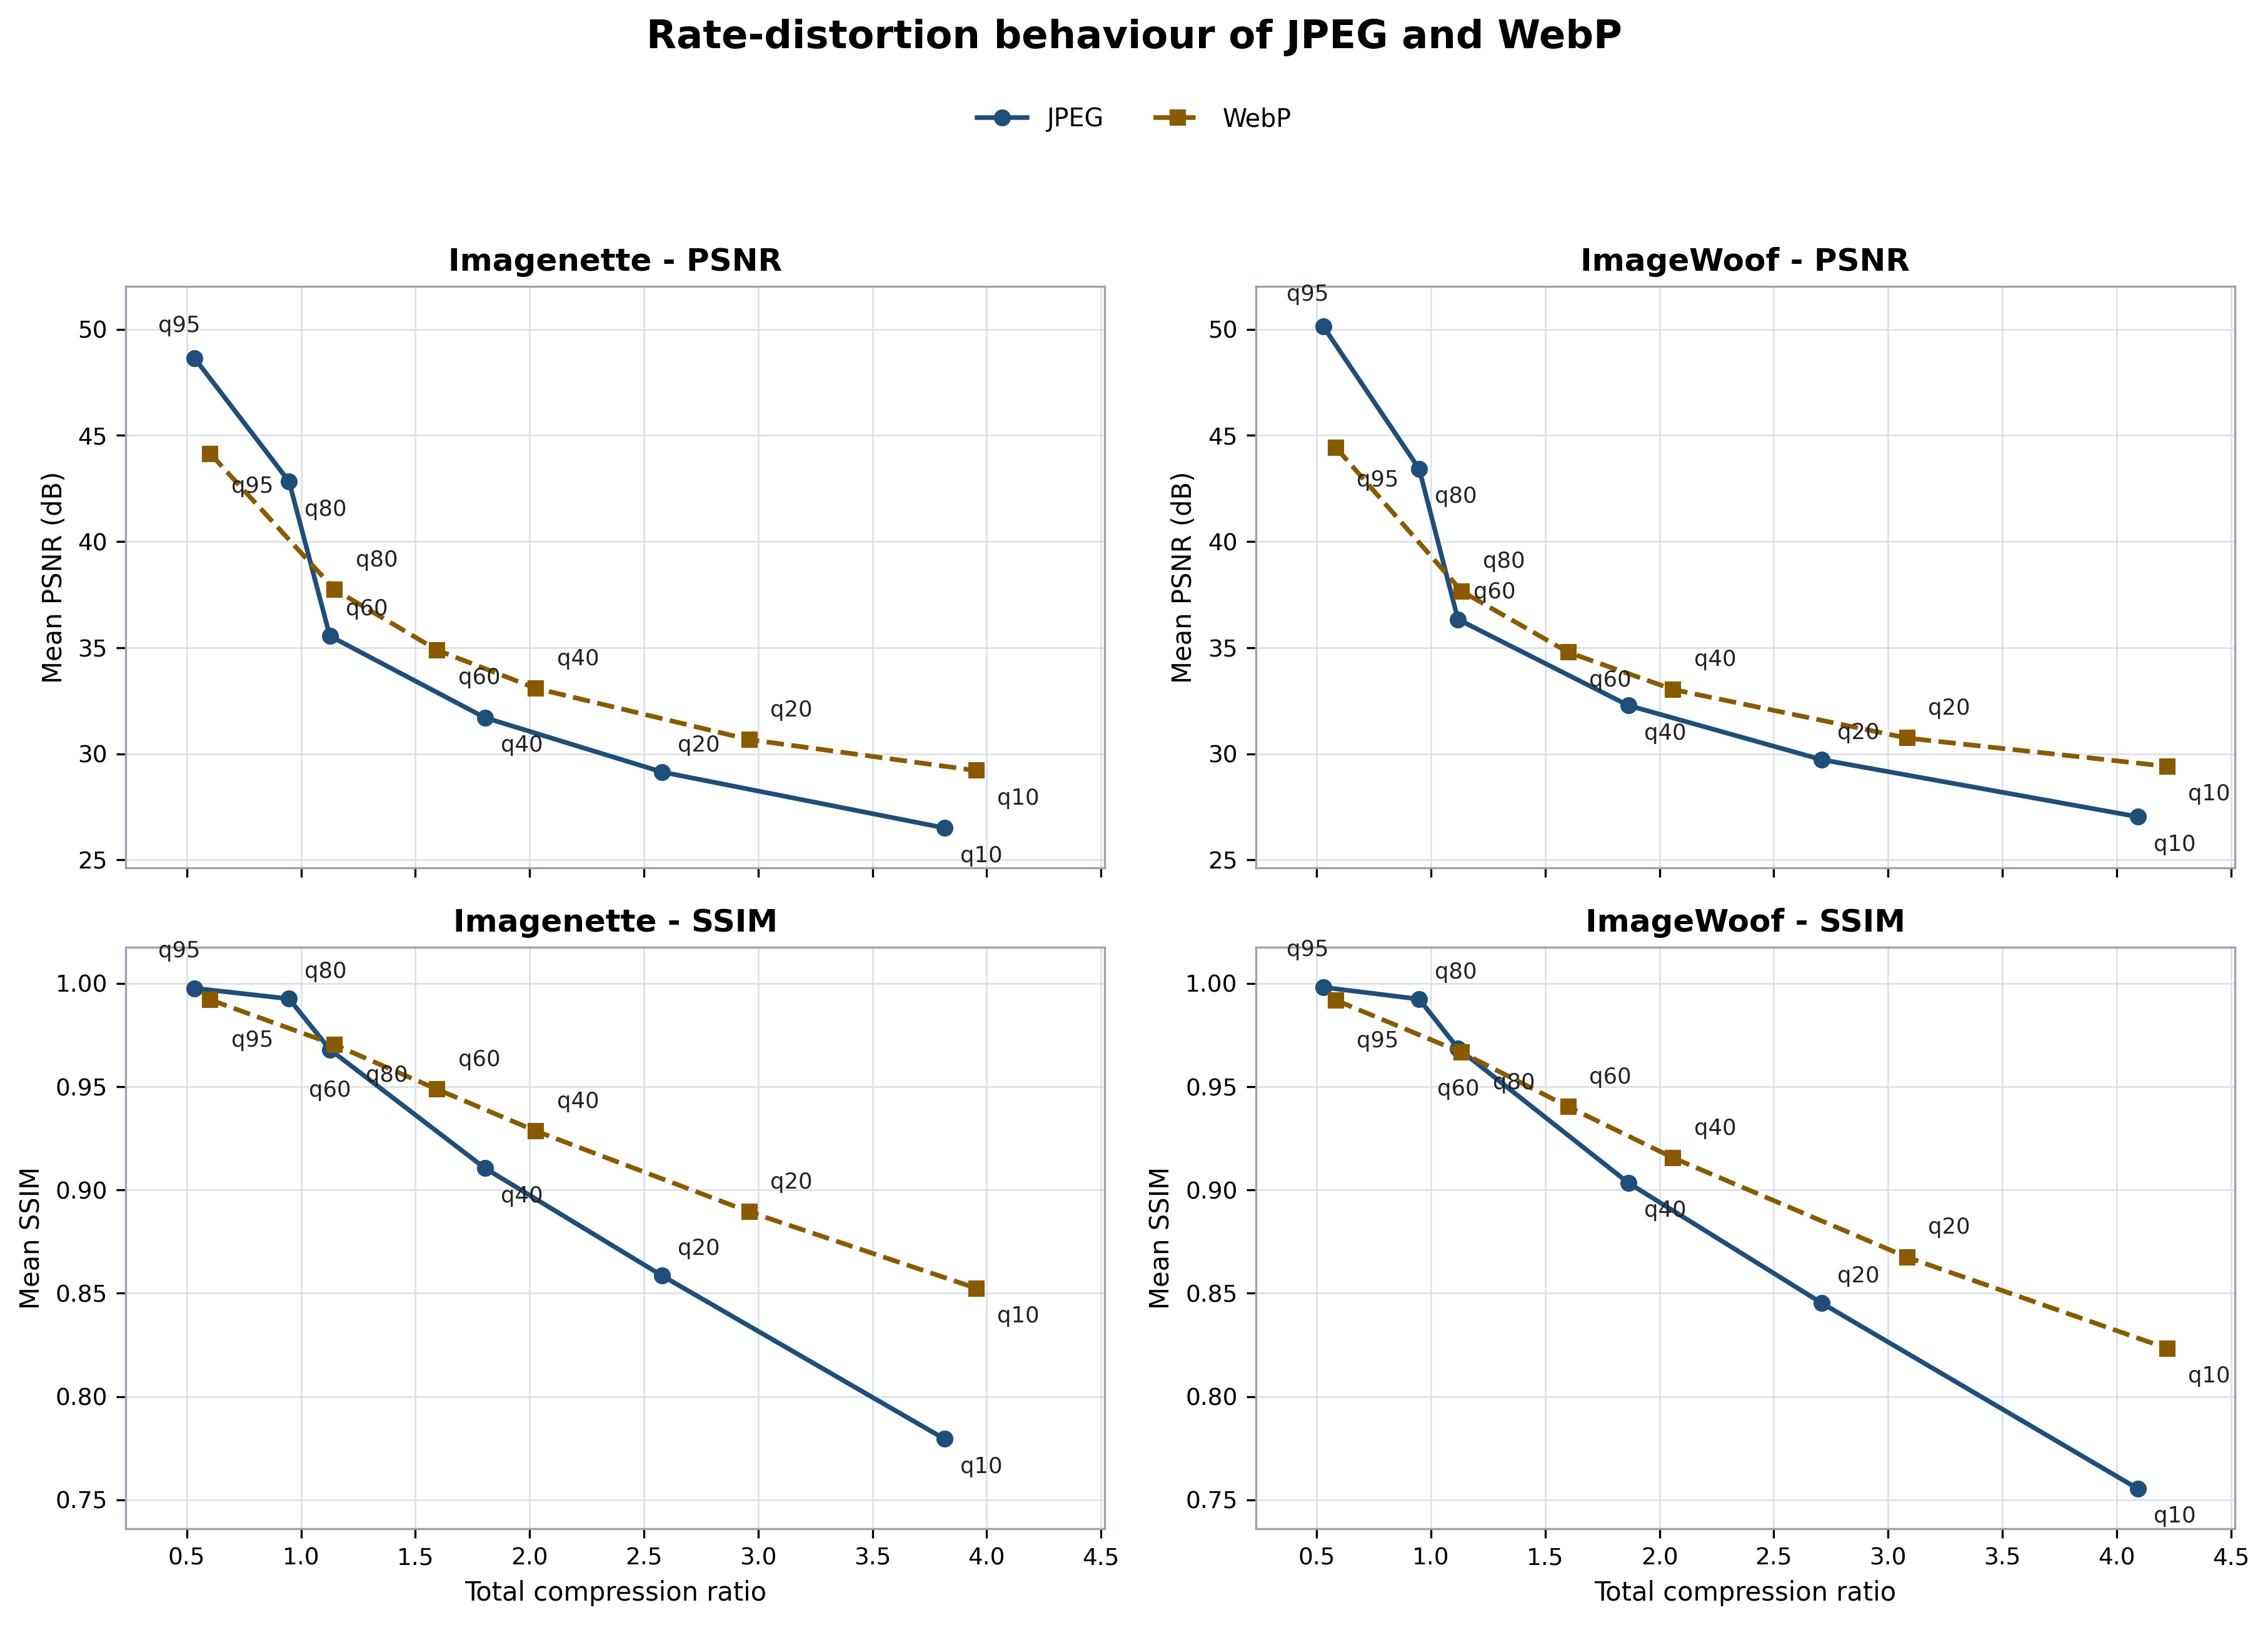
\includegraphics[width=0.82\textwidth]{../results/analysis/plots/rate_distortion_tradeoff.png}
    \caption{Mean PSNR and SSIM as functions of total compression ratio for JPEG recompression and WebP transcoding. Both metrics compare the decoded compressed image with the decoded distributed JPEG source image.}
    \label{fig:rate_distortion}
\end{figure}

\FloatBarrier

Figure~\ref{fig:rate_distortion} shows the expected rate--distortion relationship: mean PSNR decreases as compression becomes stronger, and mean SSIM also decreases as compression becomes stronger. This pattern appears for both datasets and both codecs. At stronger, approximately comparable compression ratios, the observed WebP curves generally retain higher mean PSNR and SSIM than JPEG, but this should not be interpreted as universal codec superiority. Considered together with Figure~\ref{fig:rate_accuracy}, the distortion results show why decoded image distortion and downstream classification performance should be evaluated jointly. For example, on ImageWoof, JPEG q60 has mean SSIM of approximately 0.9685 and an accuracy change of $-1.58$ percentage points, while WebP q80 has mean SSIM of approximately 0.9665 and an accuracy change of $-0.74$ percentage points. JPEG q60 therefore has a marginally higher mean SSIM in this comparison, but a larger classification loss. WebP q80 also has higher mean PSNR in the same comparison. This observation indicates that a higher aggregate SSIM does not necessarily imply better preservation of classifier performance. The spatial location and semantic relevance of the distortion may matter, but the current aggregate analysis does not directly test that mechanism.

\subsection{Targeted Threshold Refinement}

The exploratory analysis showed that the relevant accuracy-loss transition occurred in different quality regions for JPEG and WebP. This motivated the targeted evaluation of JPEG q70 and WebP q77 on both datasets. Both settings were evaluated to examine the region around the predefined 1 percentage-point tolerance. These quality values are codec-specific and should not be interpreted as equivalent settings.

\begin{table}[!htbp]
\centering
\small
\setlength{\tabcolsep}{3.5pt}
\resizebox{\textwidth}{!}{%
\begin{tabular}{lcrrrrrrl}
\toprule
Codec & Quality & Compression ratio & Size reduction & Accuracy & Accuracy loss & PSNR & SSIM & 1 pp \\
\midrule
JPEG & 70 & 1.03$\times$ & 3.2\% & 86.75\% & 0.43 pp & 41.50 dB & 0.9901 & Pass \\
WebP & 77 & 1.27$\times$ & 21.1\% & 86.06\% & 1.12 pp & 36.82 dB & 0.9645 & Fail \\
\bottomrule
\end{tabular}
}
\caption{Targeted refinement results for Imagenette.}
\label{tab:imagenette-refinement}
\end{table}

\begin{table}[!htbp]
\centering
\small
\setlength{\tabcolsep}{3.5pt}
\resizebox{\textwidth}{!}{%
\begin{tabular}{lcrrrrrrl}
\toprule
Codec & Quality & Compression ratio & Size reduction & Accuracy & Accuracy loss & PSNR & SSIM & 1 pp \\
\midrule
JPEG & 70 & 1.03$\times$ & 2.9\% & 87.55\% & 0.71 pp & 42.35 dB & 0.9913 & Pass \\
WebP & 77 & 1.26$\times$ & 20.5\% & 87.25\% & 1.02 pp & 36.72 dB & 0.9596 & Fail \\
\bottomrule
\end{tabular}
}
\caption{Targeted refinement results for ImageWoof.}
\label{tab:imagewoof-refinement}
\end{table}

\begin{figure}[!htbp]
    \centering
    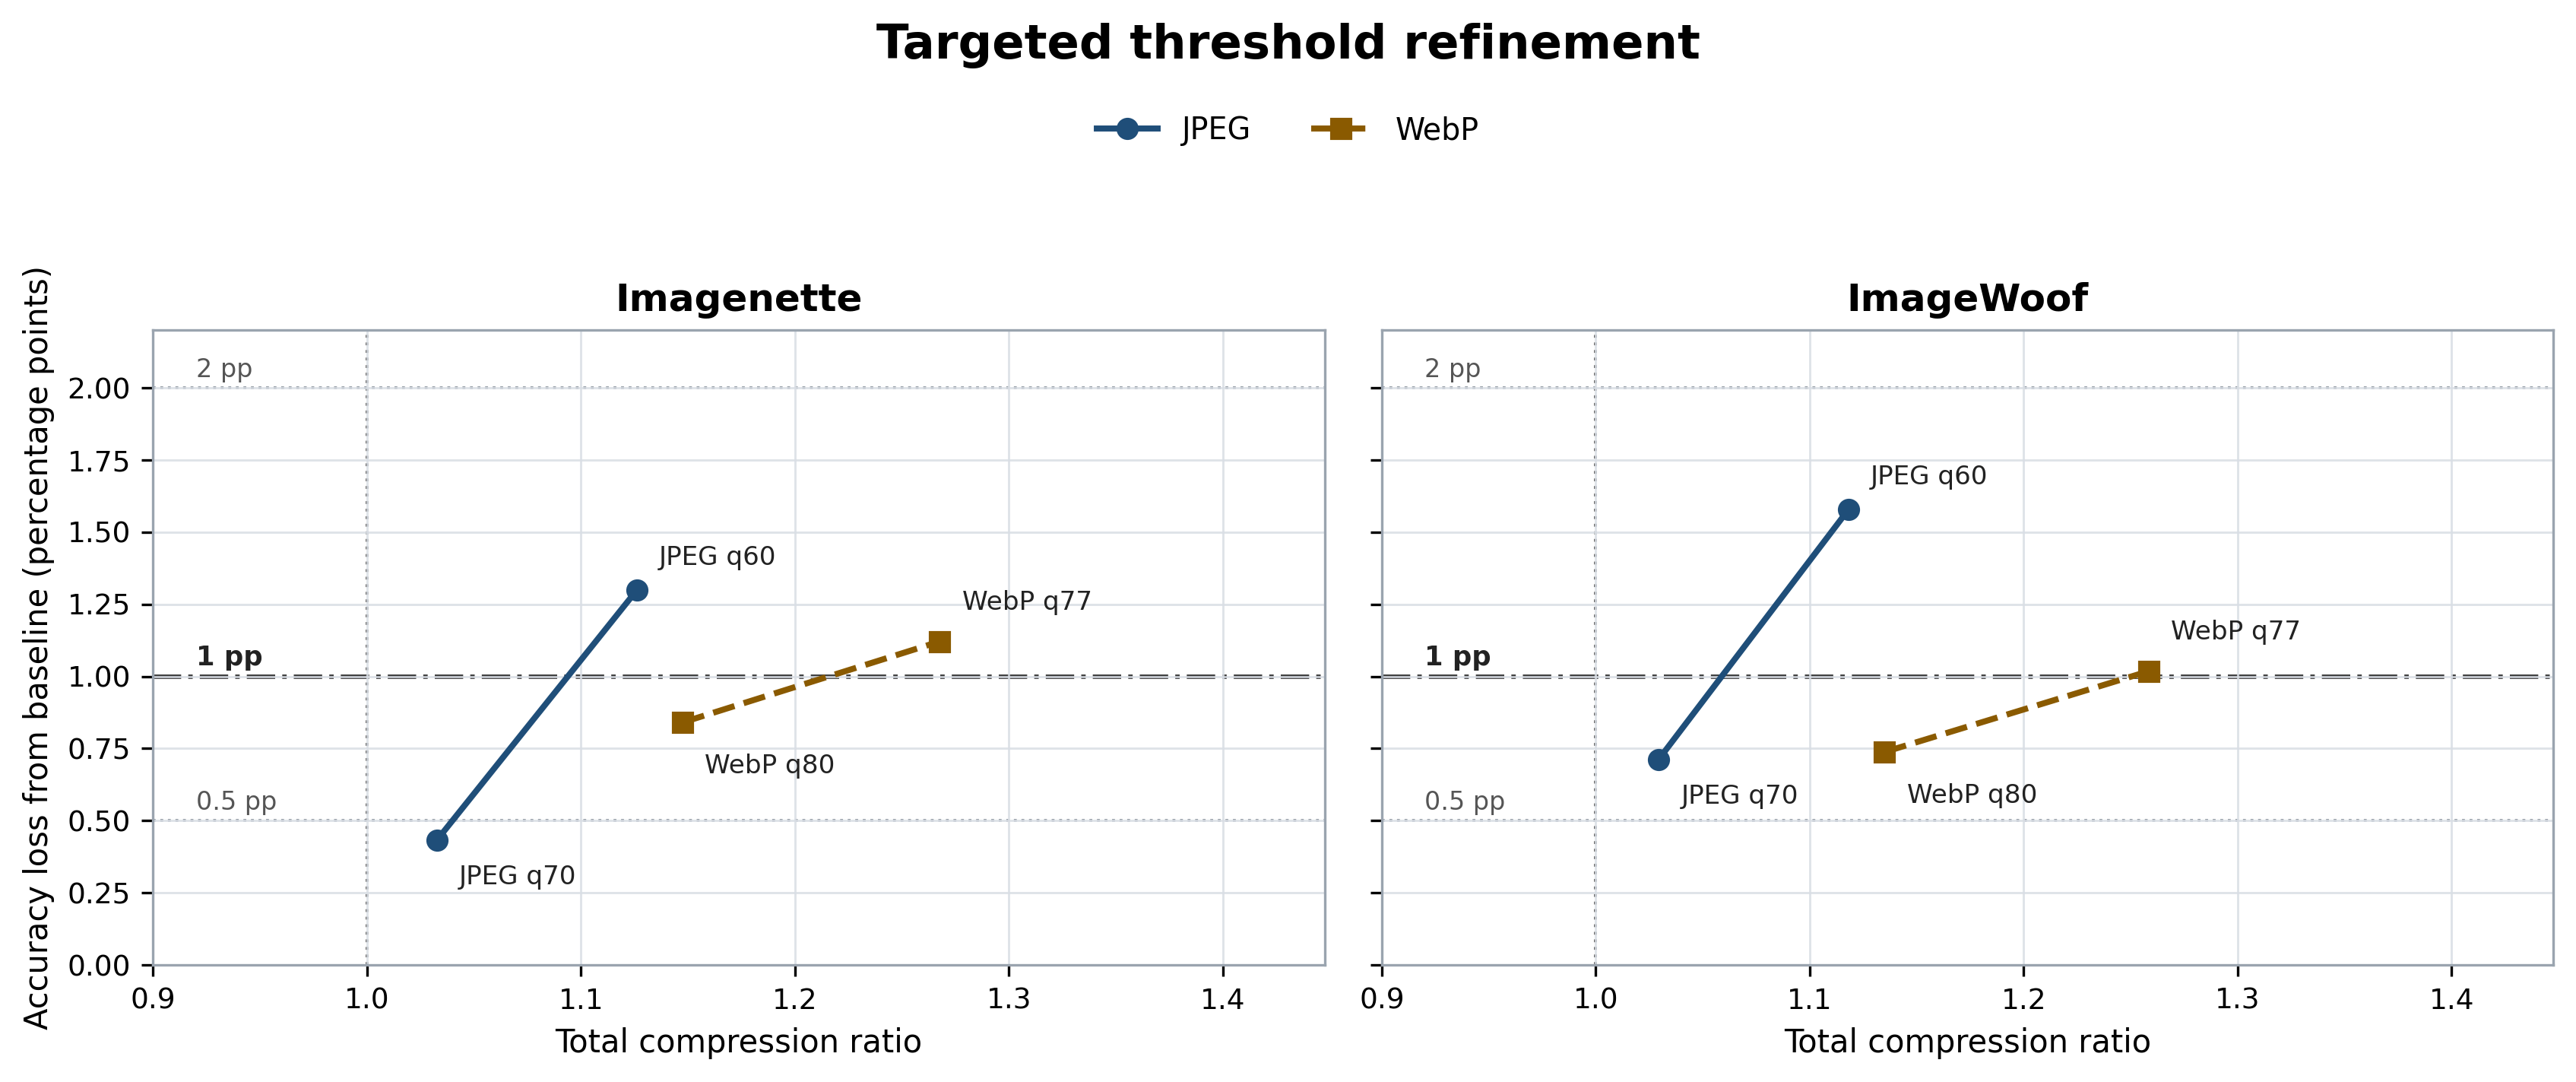
\includegraphics[width=0.87\textwidth]{../results/analysis/refinement/threshold_refinement.png}
    \caption{Targeted rate--accuracy refinement around the predefined tolerance region. JPEG q70 and WebP q77 are compared with the adjacent exploratory reference settings. The primary acceptable loss is 1 percentage point, with 0.5 and 2 percentage points shown as sensitivity margins.}
    \label{fig:threshold-refinement}
\end{figure}

Tables~\ref{tab:imagenette-refinement} and~\ref{tab:imagewoof-refinement}, together with Figure~\ref{fig:threshold-refinement}, show that JPEG q70 passes the primary tolerance on both datasets. It achieves high mean SSIM, approximately 0.99, and accuracy losses of 0.43 percentage points on Imagenette and 0.71 percentage points on ImageWoof. However, it reduces total size by only approximately 3\%. JPEG q60 provides greater storage reduction but exceeds the 1 percentage-point tolerance on both datasets. JPEG q70 is therefore the strongest tested JPEG condition satisfying the primary tolerance.

WebP q80 had already passed the primary tolerance on both datasets in the exploratory stage. WebP q77 was tested as a stronger compression point. It increases total size reduction to approximately 20--21\%, and mean SSIM remains relatively high, approximately 0.96. However, q77 slightly exceeds the primary tolerance, with an accuracy loss of 1.12 percentage points on Imagenette and 1.02 percentage points on ImageWoof. It must therefore be marked as failing the strict primary rule, while still being an informative near-boundary operating point. On ImageWoof, one changed prediction among 3,929 evaluated images corresponds to approximately 0.025 percentage points, so the difference between 1.00 and 1.02 percentage points is approximately at the resolution of one prediction. The fail designation is rule-based and should not be interpreted as evidence of a practically meaningful performance discontinuity at the 1 percentage-point boundary.

The observed points suggest that the candidate WebP operating interval lies between q80 and q77. WebP q80 reduces size by approximately 12--13\%, remains within the 1 percentage-point accuracy-loss tolerance, and retains SSIM close to 0.97. WebP q77 reduces size by approximately 20--21\%, retains SSIM close to 0.96, and exceeds the accuracy tolerance only slightly. The q77--q80 interval therefore defines a narrow and promising practical operating region. This interval offers a favourable trade-off between storage reduction, structural similarity, and classification preservation. An untested intermediate quality within this interval could plausibly provide a compromise between the two observed endpoints, but the exact operating point within this interval was not estimated because intermediate qualities were not evaluated.

\FloatBarrier

At the approximately matched storage reductions examined in this experiment, WebP obtains slightly greater storage reduction with lower classification loss. On Imagenette, JPEG q60 reduces size by 11.2\% with 1.30 percentage points loss, while WebP q80 reduces size by 12.9\% with 0.84 percentage points loss. On ImageWoof, JPEG q60 reduces size by 10.6\% with 1.58 percentage points loss, while WebP q80 reduces size by 11.9\% with 0.74 percentage points loss. Achieving a similar level of storage reduction through JPEG recompression required accepting a larger classification loss on both datasets. This is one of the principal codec-comparison findings of the study.

\clearpage
\section{Discussion}

\subsection{RQ1: Effect of Increasing Compression}

The results show that stronger useful compression generally produces greater degradation in classification accuracy, although the relationship is not perfectly linear. Some high-quality recompression or transcoding settings increase file size because the source images are already JPEG encoded, so high codec quality does not necessarily produce useful compression. Once compression ratios exceed one, classification losses generally increase as compression becomes stronger. Aggressive JPEG recompression produces particularly large losses on ImageWoof. This greater sensitivity may be related to its more fine-grained and visually similar dog categories, although the present experiment does not directly test that explanation.

\subsection{RQ2: JPEG and WebP Comparison}

JPEG and WebP quality values are not directly comparable, so the codec comparison must use compression ratio or size reduction together with classification accuracy. At approximately matched reductions, WebP preserves classification accuracy better in the tested conditions. WebP q80 offers around 12--13\% size reduction while remaining within the primary tolerance, whereas JPEG q70 passes the same tolerance but provides only around 3\% reduction. Within this experiment, WebP therefore provides the strongest observed practical trade-off, without implying that the same conclusion holds for every dataset, model, or compression implementation.

\subsection{RQ3: Practical Threshold}

The strongest tested conditions satisfying the primary 1 percentage-point rule are JPEG q70 for Imagenette, JPEG q70 for ImageWoof, WebP q80 for Imagenette, and WebP q80 for ImageWoof. These are discrete tested operating points. The observed primary-tolerance transition is bracketed by WebP q80 and q77, and by JPEG q70 and q60. These intervals describe tested operating regions rather than exact continuous boundaries. The project therefore identifies practical tested thresholds rather than mathematical continuous optima.

The selected operating point changes with the accepted loss. Under the stricter 0.5 percentage-point margin, JPEG q70 on Imagenette is the only tested size-reducing condition that remains within tolerance, while no useful tested condition passes on ImageWoof. Under the 2 percentage-point margin, the strongest tested passing points are JPEG q60 and WebP q60 on Imagenette, and JPEG q60 and WebP q77 on ImageWoof.

\subsection{Signal-Processing Interpretation}

The experiment evaluates coding rate through compression ratio and size reduction, quantization-induced decoded-signal distortion through PSNR and SSIM, and task preservation through classification accuracy. PSNR and SSIM quantify reconstruction fidelity relative to the decoded source image, while accuracy measures whether the reconstructed signal retains enough task-relevant information for the downstream classifier. A high SSIM does not guarantee that the primary accuracy tolerance is satisfied. WebP q77 illustrates this clearly: SSIM remains around 0.96, but accuracy loss crosses the 1 percentage-point boundary on both datasets. Machine-oriented compression therefore requires joint rate--distortion--accuracy evaluation.

\section{Limitations}

The study is limited to two validation sets, one frozen ResNet-50 model, and one preprocessing pipeline. Because the source images are already JPEG encoded, the experiment evaluates recompression and transcoding rather than compression from raw images. The tested quality values identify practical operating ranges rather than exact optima; a denser search could refine these ranges, but any estimated operating point would remain specific to the dataset, classifier, codec implementation, and selected tolerance. The threshold classification is based on point estimates; no paired confidence intervals, bootstrap analysis, or McNemar test were performed. Finally, aggregate accuracy, PSNR, and SSIM may hide per-class or per-image behaviour.

\section{Conclusion}

Selecting an appropriate compression operating region can reduce storage while preserving machine-classification performance. JPEG q70 is the strongest tested JPEG point passing the primary 1 percentage-point tolerance on both datasets, but it saves only about 3\%. WebP q80 is the strongest tested WebP point passing the primary tolerance, with about 12--13\% size reduction. WebP q77 increases reduction to about 20--21\%, while SSIM remains near 0.96 and accuracy loss only slightly exceeds 1 percentage point. This identifies q77--q80 as a candidate WebP operating interval, although the exact operating point within this interval was not estimated.

At the approximately matched storage reductions tested, WebP produced a smaller classification loss than JPEG. WebP therefore provides the strongest observed trade-off among rate, distortion, and accuracy in this study. The result is specific to the tested datasets, model, codec implementation, and chosen tolerance.


\clearpage
{\small
\section{References}
\makeatletter
\renewcommand{\section}{\@ifstar\@gobble\@gobble}
\makeatother
\bibliographystyle{IEEEtran}
\bibliography{references}
}

\end{document}
